\subsection{K-means}
K-means is used to group the dataset into categories depending on their location in the x-dimensional space determined by the amount of features representing one of them.
The center of these clusters are then computed and identified as a specific category.
Using these centres, a unknown element can then be categorized depending on which cluster is the closest.

To find the number of clusters best representing the dataset, then the within-group heterogeneity and homogeneity was computed for various K's as seen on figure \textbf{ref!!}.
The elbow point can from here be determined to be at \textbf{K = something}.

\begin{figure}
\centering
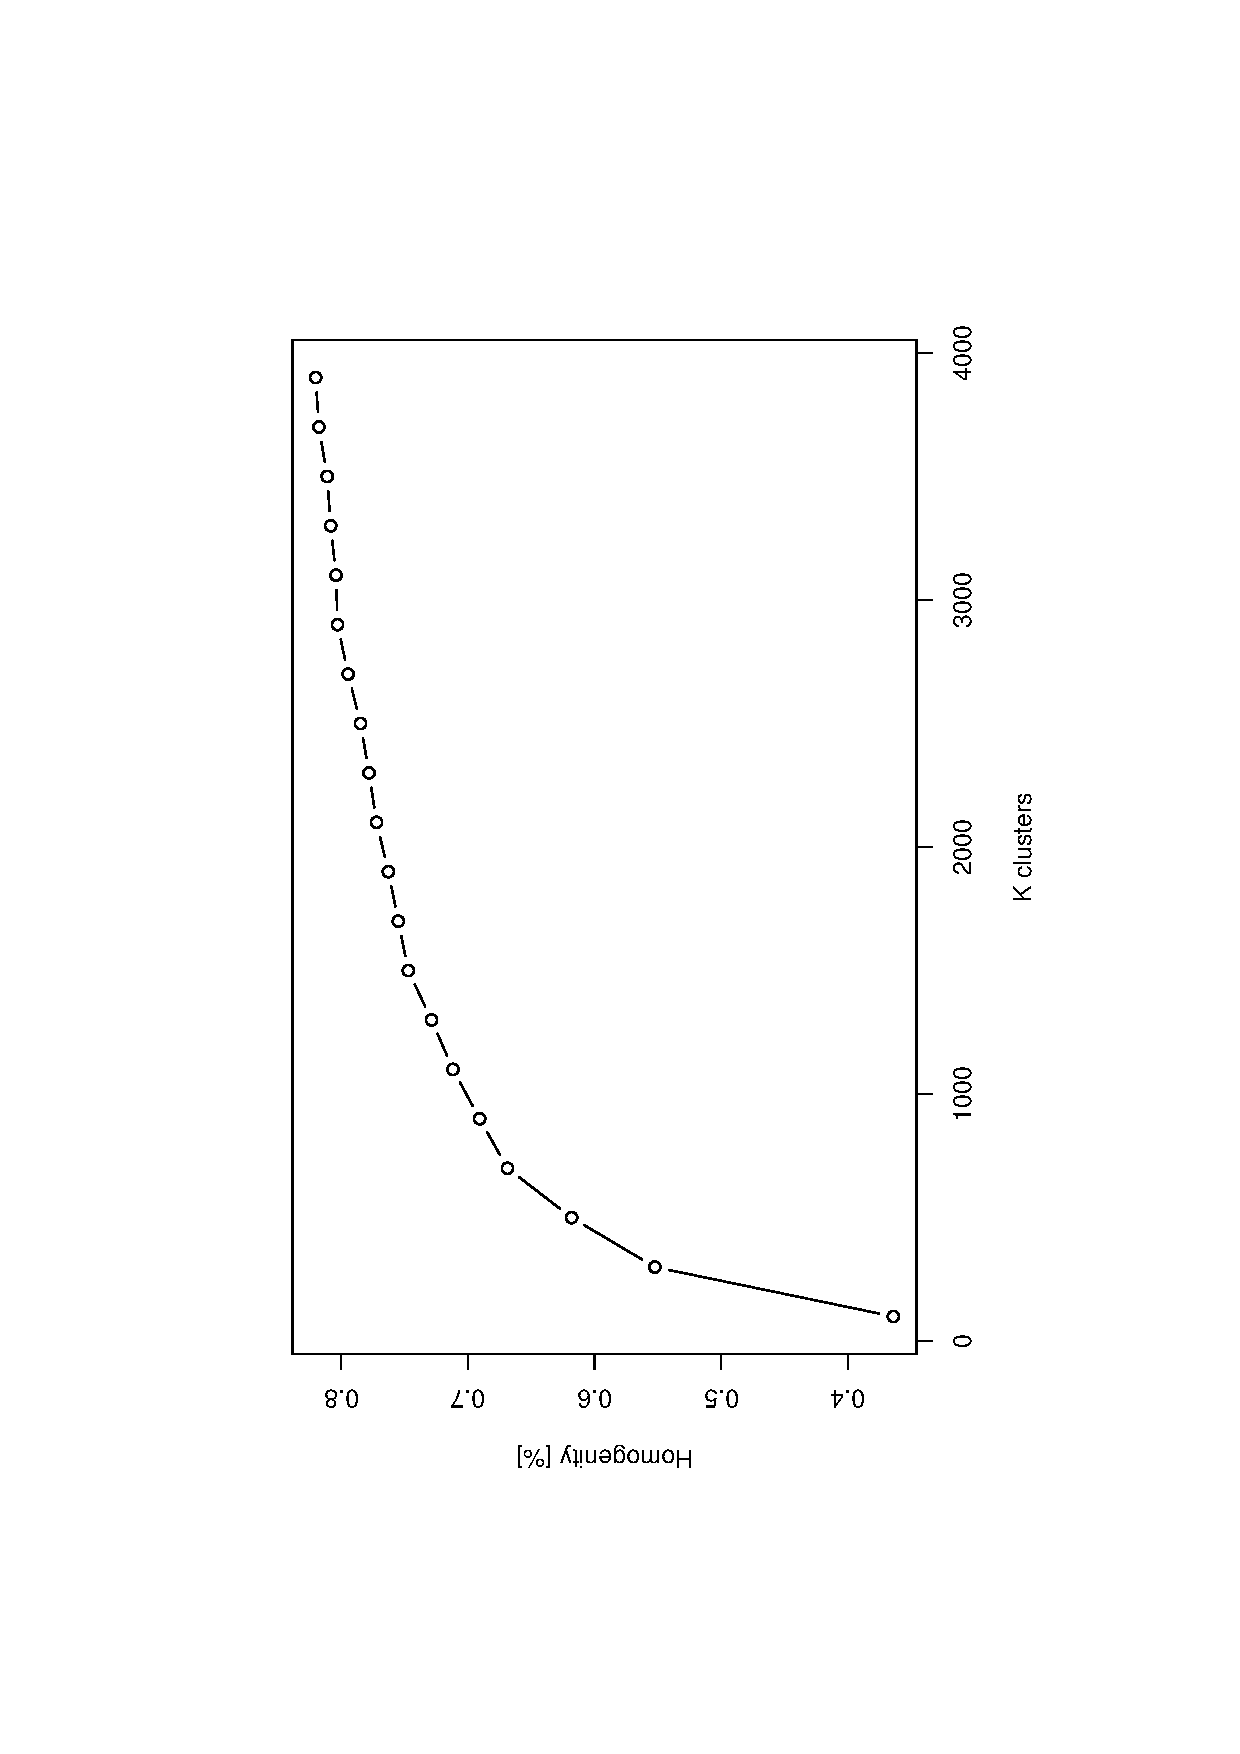
\includegraphics[width=\textwidth]{graphics/homogenity}
\caption{Homogeneity of the data set.}
\label{fig:homogeneity_kmean}
\end{figure}


\begin{figure}
\centering
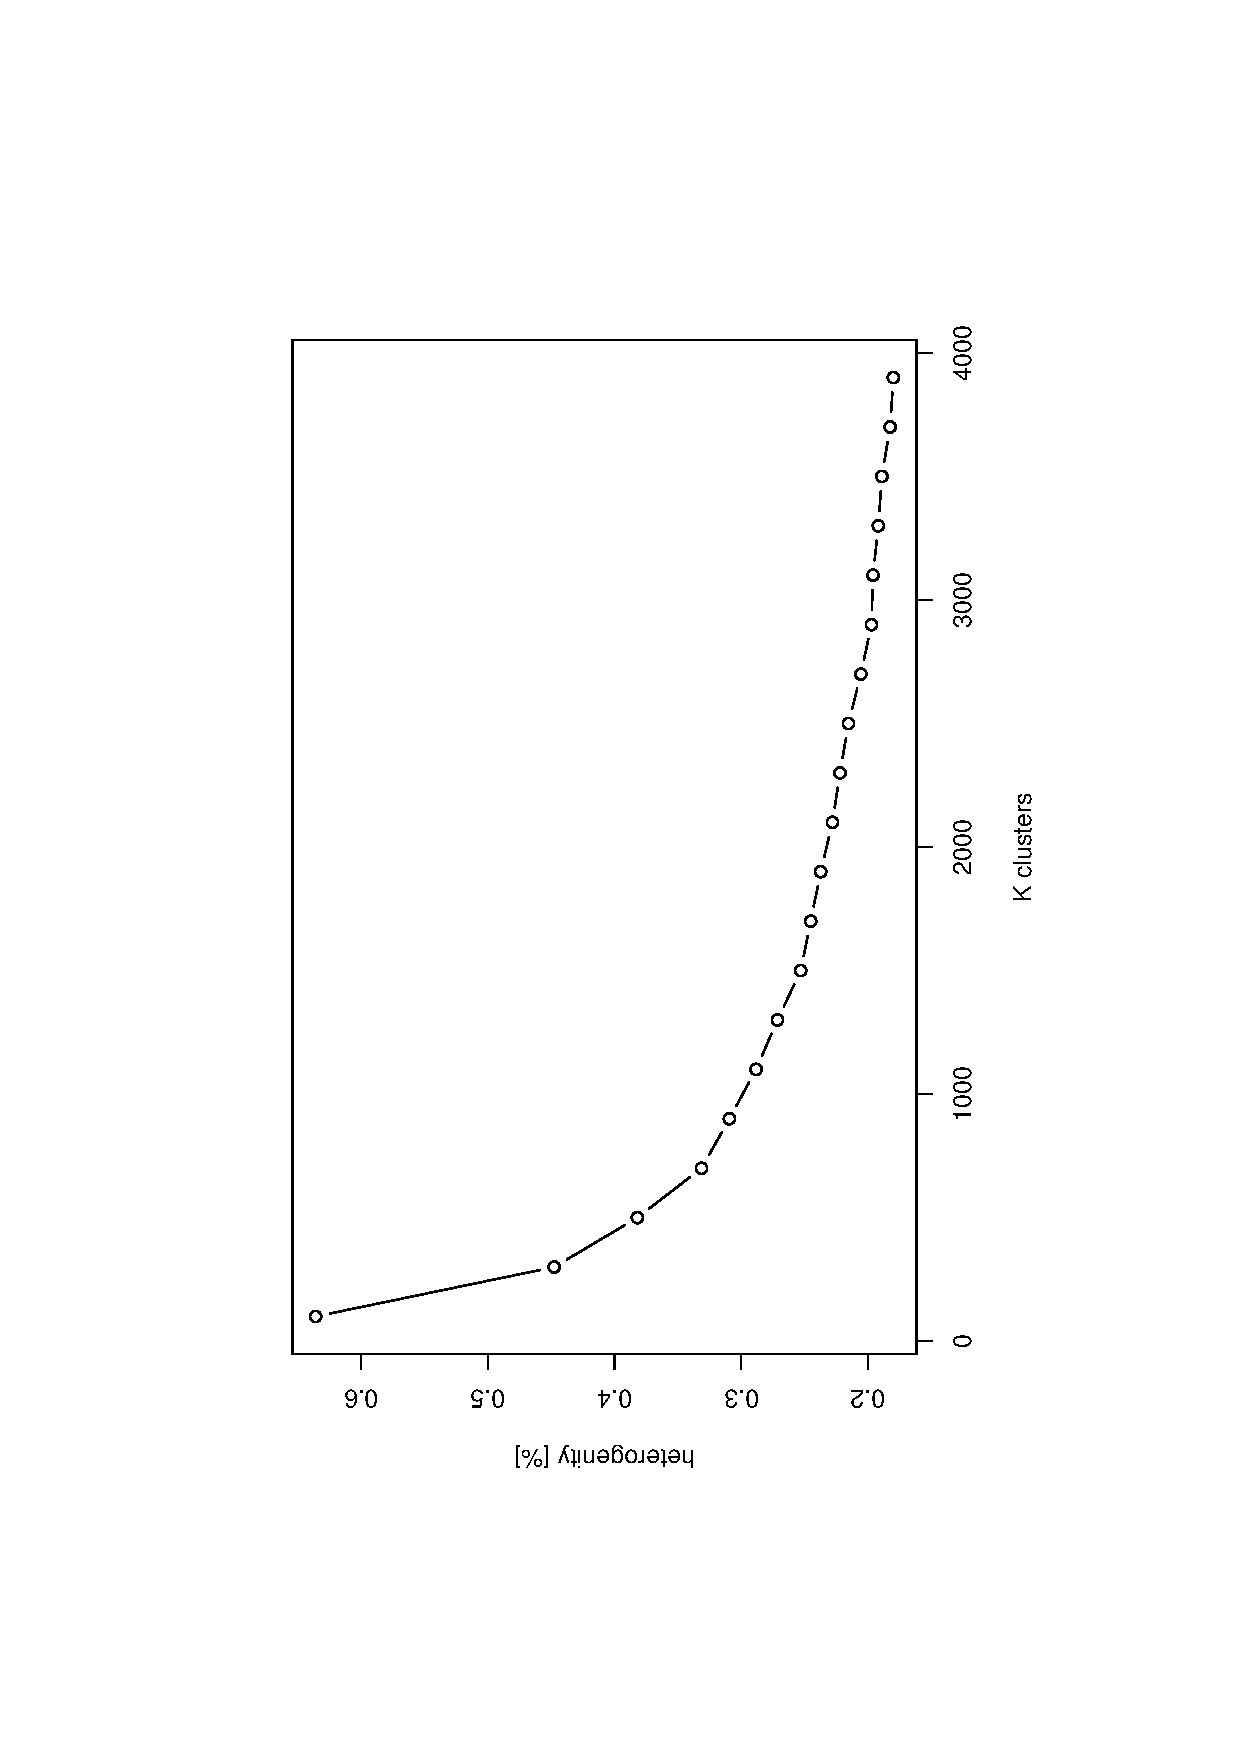
\includegraphics[width=\textwidth]{graphics/heterogenity}
\caption{Heterogeneity of the data set.}
\label{fig:heterogeneity_kmean}
\end{figure}

\begin{table}[H]
\centering
%# kmean = 400
%# k_knn = 10
%# k_mean = 10
%# kmean_iterations = 500
%# Time taken to prep kmean: 272.61"
%# [1] "Time taken to run kmean classification: 8.47000000000003"
%# [1] "Success for kmean: 0.4415"
%# [1] "Time taken to run raw knn classification: 1857.24"
%# [1] "Success for raw knn: 0.739"
\begin{tabular}{|l|r|r|}\hline
Criteria & Raw KNN & K-mean K-NN \\ \hline
Pre-Processing Time & 0s & 4m32.61s \\ \hline
Classification Time & 30m57.24s & 8.47s \\ \hline
Success Rate & 73.9\% & 44.2\% \\ \hline
\end{tabular}
\caption{Processing time comparison of running K-NN on K-mean data and raw}
\label{tab:processingtime_kmean_vs_raw_knn}
\end{table}